\section{车牌定位}
\subsection{由Viola and Jones 的face detection framework 衍生的一些方法}
\subsubsection{Viola and Jones 的Robust Real-Time Face Detection论文简述}
Viola and Jones 的人脸检测系统的主要贡献有三个:
\begin{enumerate}
\item
提出"Integral Image"的概念,提高了detector的计算速度。
\item
使用Adaboost学习算法从大量的可能特征中筛选出少量的重要的特征,以实现一个简单而有效的分类器。
\item
将分类器级联,使得显然的非人脸区域很快地被丢弃,而后面的分类器可以致力于区分那些更可能是人脸的区域。
\end{enumerate}
他们首先选择了一些相当简单的特征(features, reminiscent of Haar basis functions),他们认为,使用特征而不直接使用像素信息的重要原因是特征可以给出一些ad-hoc domain knowledge,而直接使用像素信息很难获得这些知识。另一方面,feature-based system比起pixel-based system也快得多。特征的示例见下图,他们使用的都是规则的长方形特征,特征的值为子窗口中黑白区域的像素值之和的差值。
\begin{figure}[H]
    \centering 
    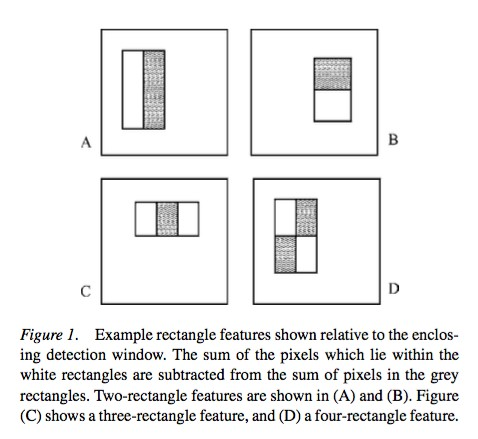
\includegraphics[width=0.618\textwidth]{image/2_1_1_1.jpg}    
    \label{logic}
\end{figure}
对每一张待检测照片,计算出它的Integral Image,就可以很迅速地计算出每个检测子窗口上的各个特征的值。他们在总结中提到,为了实现真正的尺度不变性,几乎所有的人脸检测系统都需要对每一张待检测图片的多个尺度进行检测。使用Integral Image,就可以通过改变窗口大小、保持检测图片大小不变的方式,快速地对一张图片的各个尺度进行检测。

为了提高检测系统的鲁棒性,配合Adaboost算法,首先生成一个非常巨大的矩形特征集。对于每一个特征,生成一个弱分类器:选择使得误判的样例数最少的阈值生成一个二元分类器。


然后使用Adaboost算法,选择非常少的弱分类器。Adaboost算法逐个选择加权误差最小的弱分类器,并且每添加一个特征,就更新样例的权重,使得被错误分类的样例获得更高的权重。最后生成一个强二元分类器,是选择出来的弱分类器的线性组合。Adaboost算法如下:
\begin{figure}[H]
    \centering 
    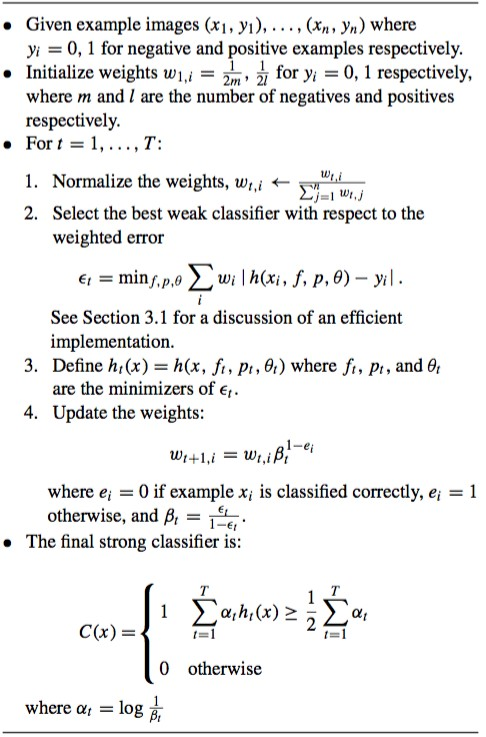
\includegraphics[width=0.618\textwidth]{image/2_1_1_2.jpg}    
    \label{logic}
\end{figure}
其中,弱分类器的选择可以使用这样的算法:

对于每一个特征,将样例按照特征的值排序,
对于每一个排好序的样例,维护4个值:所有正样本的权重之和$T^+$,所有负样本的权重值和$T^-$,排在当前样例之前的正样本的权重之和$S^+$与排在当前样例之前的负样本的权重之和$S^-$。那么,以当前样例的特征的值作为阈值的弱分类器的误差为:
$$e = \min(S+ + (T^- - S^-), S^-  + ( T^+ - S^+))$$
这样,每次选择最优弱分类器的时间复杂度为O(NK), N为样本数,K为总特征数。
另外,也可以证明adaboost算法的训练误差是可以被控制的:
\begin{figure}[H]
    \centering 
    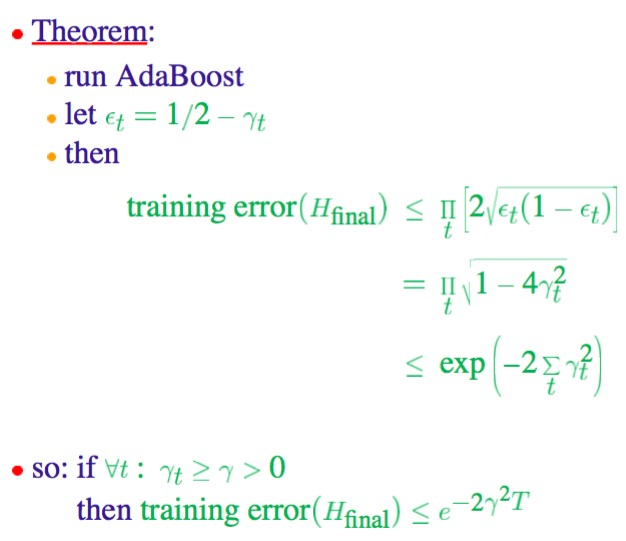
\includegraphics[width=0.618\textwidth]{image/2_1_1_3.jpg}    
    \label{logic}
\end{figure}
其中,T为最终选择的特征的个数。

作者认为,Adaboost算法的关键优势在于它学习的速度,在于每一轮选择特征时,算法将已选择的特征的信息编码到了样例的权重中。

另外,该系统使用了级联使用Adaboost得到的分类器,以提高检测能力并且减少计算时间。级联分类器的核心思想是首先使用更小的、更快速的分类器拒绝掉尽可能多的非人脸子窗口(在扫描过程中,绝大多数的子窗口中没有人脸),同时保留几乎所有的人脸子窗口(通过降低分类器的阈值),之后,使用更复杂的分类器来达到低false positive rates。决策的总体过程使用的是退化的决策树的形式,作者称其为“级联”。另外,后面的分类器接受训练时使用的是被前面的分类器所接受的样例(其中的非人脸样例更难区分),这样,他们可以解决更难的分类问题。级联分类器的运作过程如下图所示。
\begin{figure}[H]
    \centering 
    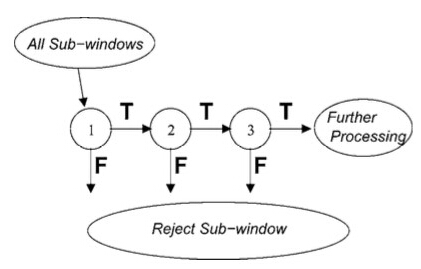
\includegraphics[width=0.618\textwidth]{image/2_1_1_4.jpg}    
    \label{logic}
\end{figure}
级联检测器的训练算法如下图所示:
\begin{figure}[H]
    \centering 
    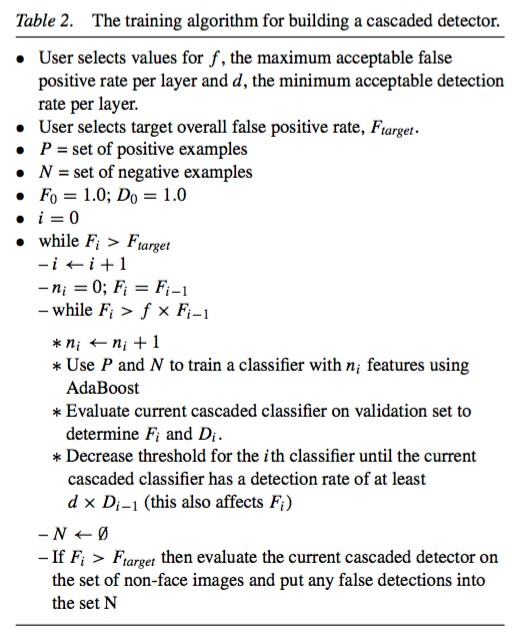
\includegraphics[width=0.618\textwidth]{image/2_1_1_5.jpg}    
    \label{logic}
\end{figure}
最后,Viola和Jones在论文的结论中提到,初步的实验表明,其他物体的高效的检测器,如行人、车辆,也可以通过这种方式构建。
\subsubsection{Chen 和 Yuille的Detecting and Reading Text in Natural Scenes}
在这篇论文中,针对城市中随意拍摄到的文本,Chen和Yuille利用Viola 和 Jones的算法框架,根据文本区域的特征分析,选择了一些特征,送到AdaBoost machine中,获得级联的Adaboost分类器。最后使用商业OCR软件阅读文字。获得了超过90\%的正确率。

作者认为,特征集的选择对算法的成功与否与透明性至关重要。由于不同文本之间的空间差异性远远强于人脸,例如眼睛在人脸上的位置是相似的,不同人的眼睛也有一定相似性,而字母的位置、形状在不同文本中差异很大。通过PCA分析,文本有更多的非零特征值,文本需要150个components才能获得90\%的variance,而人脸只需要15个components。

同时,作者强调,我们应该选择富有意义的、能传达出信息的特征,并且他们在不同的文本区域上可以得到相似的结果(低熵值,low entropy)。他们分析了文本区域的统计特征,得到如下一些结论。首先,如下图所示,文本的x, y方向上的导数的平均数、方差:
\begin{figure}[H]
    \centering 
    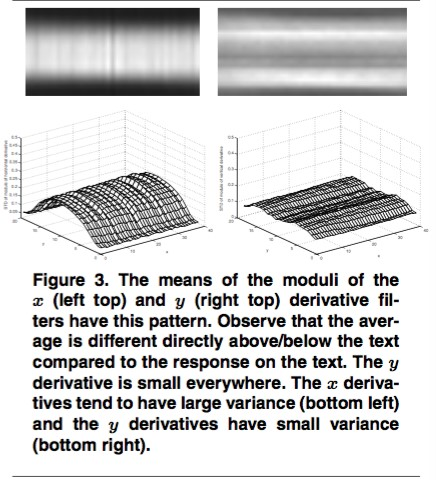
\includegraphics[width=0.618\textwidth]{image/2_1_1_6.jpg}    
    \label{logic}
\end{figure}
他们发现,x方向上的导数值在中间区域比较大,而y方向上的导数值在顶部与底部比较大,x方向上的导数值的方差在中间区域比较大,而y方向上的方差普遍比较小(低熵值)。

他们选择的第一类特征基于上述观察结果,设计了对应于x, y方向上导数的块状特征、可以包含一个文字的对称的块状特征,特征值主要为x, y方向上导数的平均值与标准差:
\begin{figure}[H]
    \centering 
    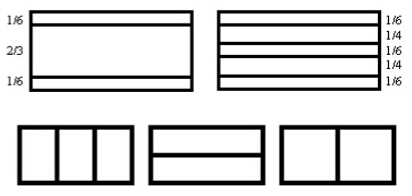
\includegraphics[width=0.618\textwidth]{image/2_1_1_7.jpg}    
    \label{logic}
\end{figure}
一个好的特征f(I)可以很好地区分两个概率分布函数P(f(I)|text)与P(f(I)|non-text),若P(f(I)|text)可以有一个很强的峰,则说明这个特征具有低熵值性。

他们选择的第二类特征基于强度、梯度方向、强度梯度值的直方图,更加复杂一些:

\begin{figure}[H]
    \centering 
    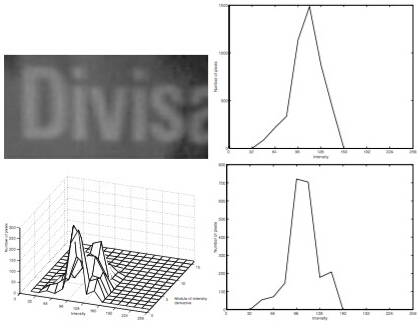
\includegraphics[width=0.618\textwidth]{image/2_1_1_8.jpg}    
    \label{logic}
\end{figure}
他们还选择了更加复杂的第三类特征,只用于级联分类器后面的阶段。第三类特征基于边缘检测,通过强度梯度阈值化、边缘连接处理。这一类特征可以计算延长的边缘的数量。具有比较低的熵值。

在使用级联的Adaboost强分类器以后,他们做了二值化操作与一些扩展操作,再将车牌送入商业OCR软件进行识别。这两步操作对我们有一定的借鉴意义。

他们首先使用了Niblack提出的自适应的二值化算法的变种(Wolf认为该算法与Yanowitz-Bruckstein的方法是最成功的二值化算法):
$$T_r(x)=\mu_r(x)+k\cdot \sigma_r(x)$$
$T_r$为阈值,$x$为像素点,$r$为一个子窗口的大小,$\mu_r$ 与 $\sigma_r$ 是该子窗口中像素值的平均值与标准差。Niblack的$r$值是固定的,作者的算法自适应地选择$r$值,因为字符的大小和笔画的粗细都不同。他们选择:
$$r(x)=\min_r(\sigma_r(x)>T_\sigma),$$
其中,$T_\sigma$是一个固定的阈值,认为标准差小于$T_\sigma$的窗口为平滑的区域。K是固定的。

作者接着使用了连通区域算法对字符区域进行扩展,因为有时使用Adaboost算法得到的字符区域是不完整的。
\subsubsection{Louka的 License Plate Detection Using AdaBoost}
Louka 的论文衡将文本提取的方法(Chen and Yuille)与人脸检测的方法(Viola and Jones) 应用到 了LPR(license Plate Recognition)系统,并对这种方法进行评估。

他提到,通过PCA分析,发现车牌需要的components比Chen和Yuille的文本要少很多,因为字体、朝向都是比较固定的。他选择特征的标准与Chen 和 Yuille 一样,希望有比较低的熵值(在所有的车牌上的检测结果比较相似),而又可以很好地区分车牌区域与非车牌区域。

他们将车牌的大小统一后,车牌x,y方向上的导数绝对值的均值与方差如下图所示:
\begin{figure}[H]
    \centering 
    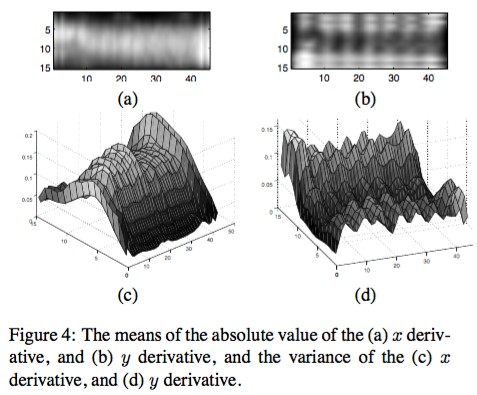
\includegraphics[width=0.618\textwidth]{image/2_1_3_1.jpg}    
    \label{logic}
\end{figure}
x方向上的导数的统计特征与Chen and Yuille的相似,而在y方向上可以明显看到车牌上7个字符到来的导数的变化。根据这一观察结果,他们选择了 Haar-like 特征,将扫描窗口水平或垂直地分为2-7个大小相等的子区域,特征值为一部分子区域上某些值的和减去剩下的子区域上的同一类值的和。示例如下图:
\begin{figure}[H]
    \centering 
    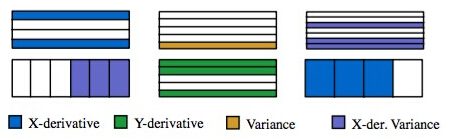
\includegraphics[width=0.618\textwidth]{image/2_1_3_2.jpg}    
    \label{logic}
\end{figure}
用于求和并相减的值为,像素强度,导数,导数方差。每个特征训练生成一个弱分类器,在这篇论文中作者使用了类条件密度来训练弱分类器,这里没有使用阈值,而是当车牌的类条件密度比非车牌条件密度的大时,判断为车牌。如下图所示:
\begin{figure}[H]
    \centering 
    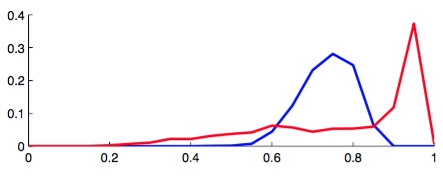
\includegraphics[width=0.618\textwidth]{image/2_1_3_3.jpg}    
    \label{logic}
\end{figure}
这里也使用了Integral Image的方法,对于像素强度,导数,倒数方差都可以计算出Integral Image,减少计算时间。方差可以由下面的公式,通过Integral Image,快速得到。
\begin{figure}[H]
    \centering 
    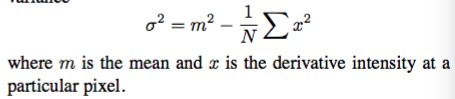
\includegraphics[width=0.618\textwidth]{image/2_1_3_4.jpg}    
    \label{logic}
\end{figure}
另外,本文使用了聚类的方法,使用每一个group的均值将检测到的包含同一车牌的临近区域进行合并。

最后,本文对错误分类的情况进行分析,并给出了一些解决方案。比如,利用比较容易检测的车尾灯,通过检测到的区域距离车尾灯的距离来进一步判断该区域是否为车牌区域。

\subsubsection{Real-Time License Plate Recognition on an Embedded DSP-Platform}
这篇论文在嵌入式DSP平台上实现了一个功能完整的车牌检测与识别系统,可以实时地从视频流中提取出车牌。主要有检测与识别两个模块,我们在车牌定位这一部分中首先描述它的检测模块。整个系统的工作示意图如下:
\begin{figure}[H]
    \centering 
    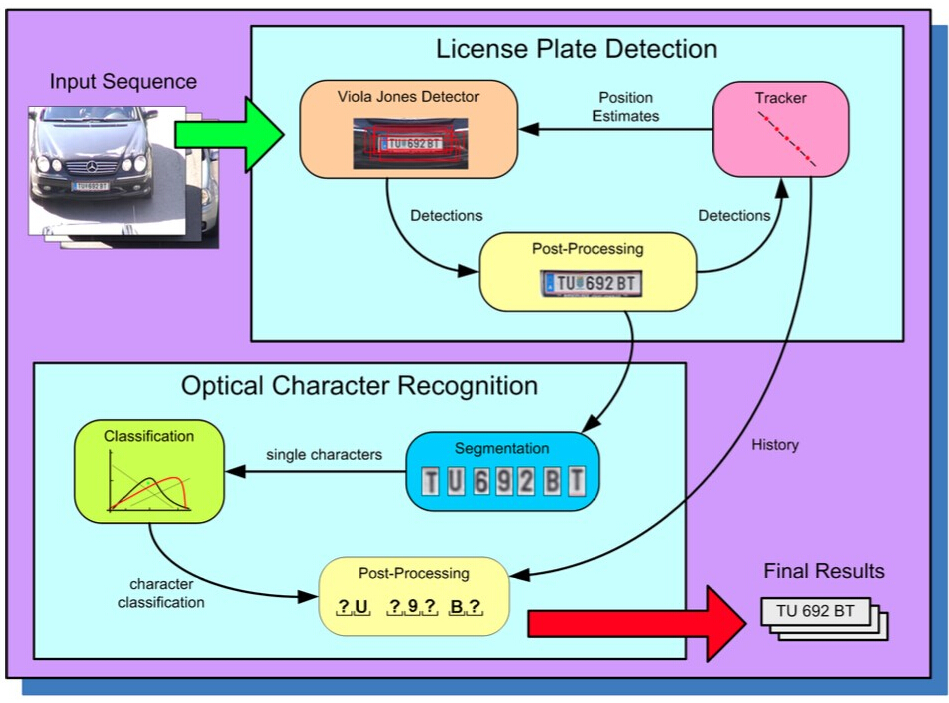
\includegraphics[width=0.618\textwidth]{image/2_1_4_1.jpg}    
    \label{logic}
\end{figure}
\paragraph{检测部分}
检测部分基于Viola 和 Jones的framework,但是根据后续的论文做了很多改进。
\begin{enumerate}
\item
使用了RealBoost算法,使用confidence rated predictions代替了二元的分类标签。
算法基本与Adaboost一致,如下图所示:
\begin{figure}[H]
    \centering 
    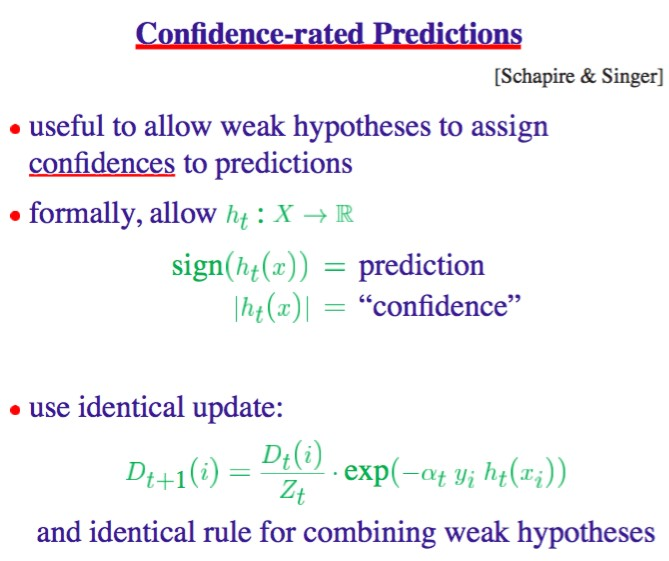
\includegraphics[width=0.618\textwidth]{image/2_1_4_2.jpg}    
    \label{logic}
\end{figure}
\item
为级联分类器添加了 inter stage feature propagation(Sochman and Matas, Inter-stage Feature Propagation in Cascade Building with AdaBoost)

这篇论文的核心思想在于,作者认为,在Viola and Jones 提出的级联算法中,每一个阶段的分类器,都生成了一个新的训练集,然后使用Adaboost算法在一个全新的问题上跑出的结果,这个分类器完全抛弃了前面的阶段中的生成的分类器。

他们认为,前一个阶段生成的分类器对于当前的新的训练集,还是可以作为当前分类器的一部分(当前分类器的起点,第一个弱分类函数),只需要调整一下阈值,因为前面的阶段为了保证不把人脸误判为非人脸,会特意调低阈值。
\begin{figure}[H]
    \centering 
    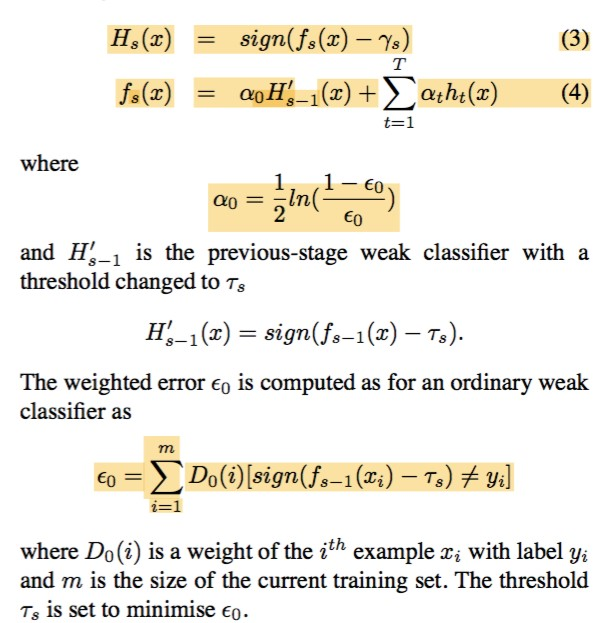
\includegraphics[width=0.618\textwidth]{image/2_1_4_3.jpg}    
    \label{logic}
\end{figure}
将前一个阶段的得到的分类器作为当前分类器的第一个弱分类器有以下原因:
\begin{enumerate}
\item
由于训练集发生了变化,而前一个阶段得到的分类器作为当前阶段的第一个弱分类器,所以每个训练样本的权重服从均匀分布,不会影响弱分类器的表现。
\item
它可以将Adaboost的学习过程集中于解决没有被前面阶段所解决的分类问题。
\item
3.	这样的分类器有一个很大的优势是,前一个阶段的$f_s(x)$都在上一阶段已经计算过了,所以$H^’_{s-1}(x)$的计算成本很低,作者称之为zero evaluation cost。
\end{enumerate}
实验表明,使用inter-stage feature后,可以使用更少的层数,达到同样的false positive rate 与 false negative rate,同时没有增加计算复杂度。而且比Viola and Jones的cascede快了25\%。
\item
特征池中增加了边沿朝向直方图特征(EOH)(Kobi Levi and Yair Weiss, Learning Object Detection from a Small Number of Examples: the Importance of Good Features.)

Levi的这篇论文致力于寻找在很小的训练集上也能表现得很好的特征。他们使用edge orientation histograms(EOH),并且证明这种特征能够达到上述目的。

EOH的示意图与其他特征的对比图如下:
\begin{figure}[H]
    \centering 
    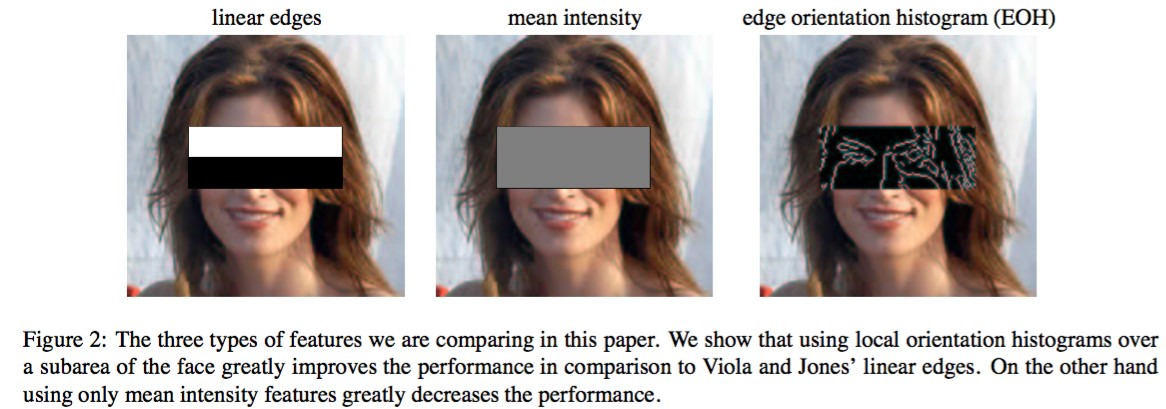
\includegraphics[width=0.618\textwidth]{image/2_1_4_4.jpg}    
    \label{logic}
\end{figure}
选择EOH的理由有:EOH与全局光照的变化无关,并且能够捕捉到前两种特征很难捕捉到的几何特性。

EOH的获得,首先使用了sobel masks,因为他们简洁并高效。若将边沿朝向分为K个组,则每个像素点获得K个特征值$(\phi_k(x, y))$:
\begin{figure}[H]
    \centering 
    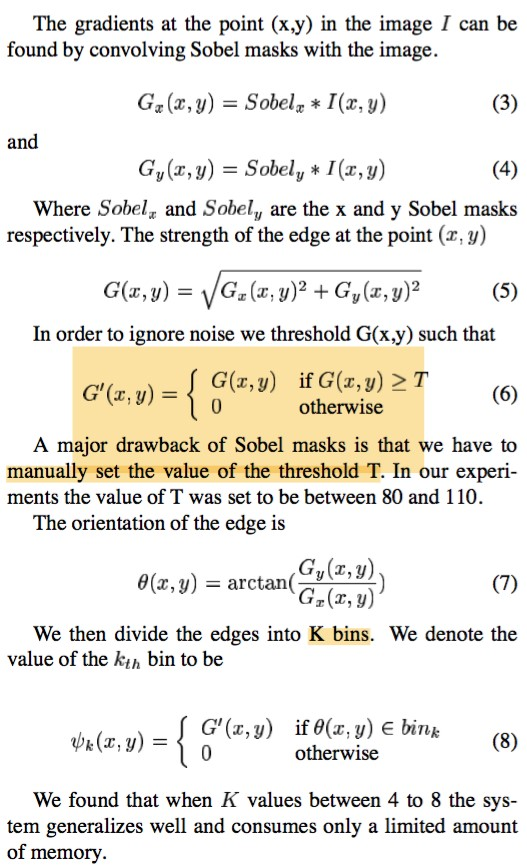
\includegraphics[width=0.618\textwidth]{image/2_1_4_5.jpg}    
    \label{logic}
\end{figure}
在每个子窗口上定义$E_k$:
$$E_k(R)=\sum_{(x,y)\in R}\Phi_k(x,y)$$
类似前面的描述,EOH特征也可以通过Integral Image的方式快速获得。接下来,论文定义了一系列EOH特征:
$$A_{k1,k2}(R)=\frac{E_{k1}(R)+\epsilon}{E_{k2}(R)+\epsilon}$$
通过设定阈值,该特征决定了,相对于k2朝向而言,k1朝向是否有决定性作用。

dominant orientation feature:
$$B_k(R)=\frac{E_k(R)+\epsilon}{\sum_iE_i(R)+\epsilon}$$

symmetry features: 
$$Symm(R_1,R_2)=\frac{\sum_{k \in K}|E_k(R_1)-E_k(R_2)|}{sizeof(R_1)}$$
实验表明,使用EOH系列特征,可以从很小的数据库(250张正面脸)中学习,并获得很好的表现。另外,论文将EOH特征作用在区分椅子的应用中,也取得了很好的效果。所以,EOH特征是一种很好的特征,可以用于多种物体的检测。
\paragraph{Post-processing 部分}
处理包含同一车牌的许多区域,使用了non-maximum suppression方法,选择confidence value最大的区域代表这一组检测到的区域。
\paragraph{Tracker部分}
一个Kalman tracker被整合到了系统中,Tracker主要用于更新并且预测同一张车牌在视频后面的帧中的位置,然后将检测器的搜索范围限定在一定的区域内,这样会比重新扫描整张图片快。另外,tracker对字符分类步骤也有很大的帮助。如下图所示:
\begin{figure}[H]
    \centering 
    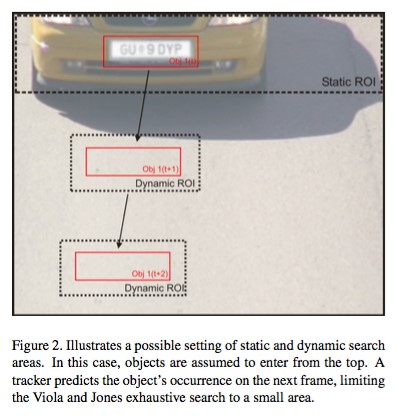
\includegraphics[width=0.618\textwidth]{image/2_1_4_6.jpg}    
    \label{logic}
\end{figure}
\end{enumerate}

\subsection{R. F. Prates, G. Cámara-Chávez, William R. Schwartz2, and D. Menotti, Brazilian License Plate Detection Using Histogram of Oriented Gradients and Sliding Windows }
在这篇论文中,作者将Dalal提出的用于人体检测的HOG算法应用到巴西车牌检测系统中去,实现了大于98\%的recall,大于78\%的precision。

整体流程见下图:
\begin{figure}[H]
    \centering 
    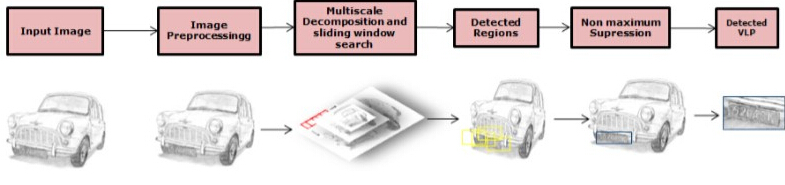
\includegraphics[width=0.618\textwidth]{image/2_2_1.jpg}    
    \label{logic}
\end{figure}
主要算法流程:
\begin{enumerate}
\item 
图像被分成若干个cell,对于每个cell,可以计算得到一张朝向梯度的直方图(HOG)。

使用1维Sobel算子得到x、y方向上的梯度:
$$dx=I(x+1,y)-I(x-1,y)$$
$$dy=I(x,y+1)-I(x,y-1)$$
接着计算magnitude与orientation:
$$m(x,y)=\sqrt{dx^2+dy^2}$$
$$\theta(x,y)=\arctan(\frac{dy}{dx})$$
\item
为了使得特征不受光照强度、对比度的影响,有效的局部对比度正规化(normalization)对于好的表现是必要的。

Cells被组成block,对于每个block进行正规化操作。Block是重叠的,所以一个cell可以属于多个block,获得不同的normalization。最后每个cell的描述符为他所从属的所有在detection window中的block的所有components所组成的向量。

这里,为了效率,选择L1-norm作为正则化的方法:
$$v'=\frac{v}{\sqrt{||v||^2_2+\epsilon^2}}$$
$v$是一个给定block中所有cell的直方图向量。
通常也会使用高斯函数,给中心的像素点更高的权重。
\item
使用magnitude与orientation,就可以构造出朝向梯度直方图。即,按照orientation放到不同的bin中,magnitude作为权重,在Dalal的论文中,为了使得介于两个bin之间的orientation可以获得更好的分类,所以会将每个像素点放到两个bin中,权重为将他的magnitude按照他的orientation到两个相邻bin的距离按比例分配。
\item
为了检测出不同尺度的车牌,对每一章图片,构造尺度不同的金字塔。
\item
对于金字塔中的每一层,使用固定大小的窗口,以固定的步长,提取出HOG特征,送到训练好的分类器中(在这篇论文中,使用的是线性的SVM)进行检测。
\end{enumerate}
\subsection{openALPR系统所使用的LBP特征}
LBP(local binary pattern)也是一种特征向量。他是这么计算的:
\begin{enumerate}
\item
将整个检测窗口分成cells(例如,16*16)
\item
对于每个cell中的每个像素,将它与它的8个相邻像素点相比较。若中心像素点的值大于邻居的,则写0,反之则写1。这样,每个像素点就有了1个8位二进制数字。
\begin{figure}[H]
    \centering 
    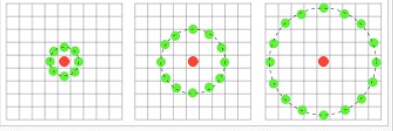
\includegraphics[width=0.618\textwidth]{image/2_3_1.jpg}    
    \label{logic}
\end{figure}
\item
对每个cell,计算直方图,即每种8位二进制数字的频率。这个直方图可以看做是256维的特征向量。
\item
可以选择性地normalize histogram。方法类似HOG特征的normalization。
\item
将检测窗口中所有cell的直方图连接起来,作为整个检测窗口的特征向量。
\end{enumerate}
获得的特征向量可以使用SVM或其他机器学习算法进行分类。

一种实用的扩展是将所有uniform pattern(如果一个local binary pattern至多只有2个0-1或1-0的变化,例如00010000)分为一类。这样,可以将每个cell的特征向量的长度从256维减少到59维。

LBP特征主要用于人脸识别与纹理分析。openALPR的开发者解释到,Haar与LBP非常相似。区别在于LBP更快一些,特别是在一些没有浮点数处理器的嵌入式设备上。Haar可能给出略微更好一些的结果,但是Haar的训练时间很慢。另外,LBP具有在所有的东西上都能工作得很好的特性,不像一些其他检测器,只能作用在黑白车牌上。
\subsection{Jiri Matas, Karel Zimmermann, Unconstrained Licence Plate and Text Localization and Recognition.}
该方法在后来被称为MSER(Maximally Stable Extremal Region)方法。该方法被认为是计算机视觉中最有趣的点检测器之一。

MSER是图片中的像素极值区域,即该区域的所有像素值均比他的外边界大(MSER+),或者该区域的所有像素值均比他的外边界小(MSER-)。MSER特征对光照变化具有不变性。

寻找MSER的线性时间算法如下:
\begin{figure}[H]
    \centering 
    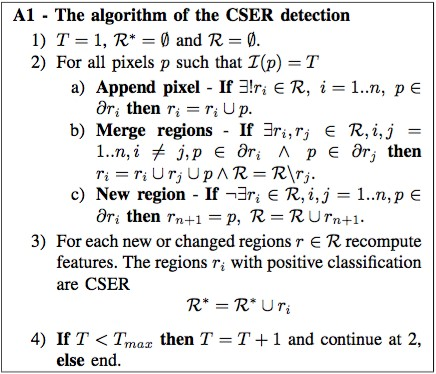
\includegraphics[width=0.618\textwidth]{image/2_4_1.jpg}    
    \label{logic}
\end{figure}
其中,I is the image and R, R∗ are set of current extremal regions (appropriate to the threshold T) and set of CSER (subset of extremal regions), respectively. 

找到了图像中所有的MSER后,这里以白底黑字的车牌为例,介绍如何定位车牌,其他类型的车牌二值化后可能需要反色来达到白底黑字的效果 。
\begin{figure}[H]
    \centering 
    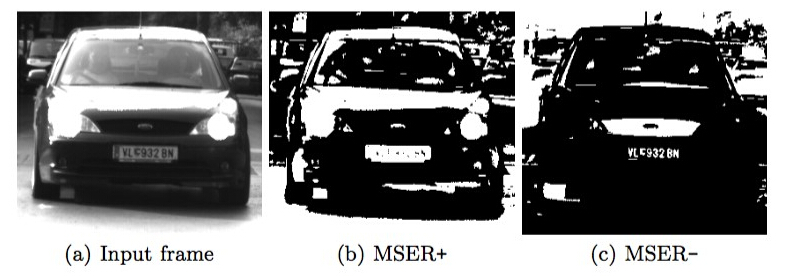
\includegraphics[width=0.618\textwidth]{image/2_4_2.jpg}    
    \label{logic}
\end{figure}
可以看到,车牌本身是一块MSER+,而他里面的字符是MSER-。所以我们寻找的是一个较大的MSER+,包含一组较小的MSER-。同时,我们制定一系列规则,来进一步筛选车牌:
\begin{enumerate}
\item
MSER-大小相近
\item
MSER-的中点几乎在一条线上(水平方向的)
\item
MSER+的高度与MSER-高度的平均值相近
\item
MSER+至少包含了3个MSER-
\end{enumerate}
这样筛选出来的MSER+就是车牌区域,而MSER-区域可以作为车牌字符分割的结果。所以MSER方法是非常高效的。
\subsection{于深洋的硕士论文《自然环境下的车牌定位与字符分割方法的研究》}
这篇论文的第三章使用了粗定位与精确定位两个阶段,组合了多种方法,实现了车牌定位。通过车牌粗定位,车牌候选区域将从图像内众多的区域中保存并突现出来;通过车牌精确定位,车牌在图像中的位置将得到更加准确的定位,而且粗定位后残留下来的伪车牌区域也将被剔除。 

车牌定位算法的整体思路简述如下:
\begin{enumerate}
\item
利用区域生长算法求得二值图像中所有的连通区域,并利用高度阈值进行筛选,删除掉过高和过矮的干扰区域。 
\begin{figure}[H]
    \centering 
    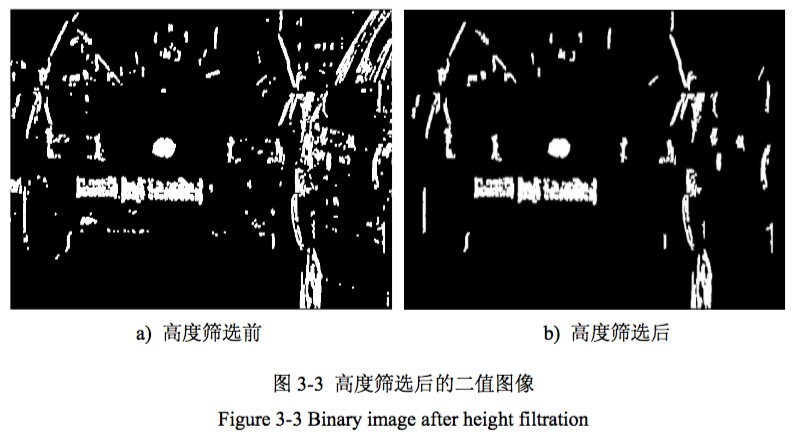
\includegraphics[width=0.618\textwidth]{image/2_5_1.jpg}    
    \label{logic}
\end{figure}
\item
对图中所有高度适合的连通区域进行水平聚类,剔除横纵比、面积、梯度密度超出阈值范围的聚类区域,这样保留下来的每个聚类区域就作为一个车牌候选区域,粗定位阶段处理完毕。 判定两区域水平相关(可以聚为一个类)的准则关系如下:
$$\left\{
\begin{aligned}
|Y^i_{Mid}-Y^j_{Mid}| & \leq \Delta y \\
X^j_{Min}-X^i_{Max} & = \leq \Delta X\\
|H_j-H_i| & = \Delta xy
\end{aligned}
\right.
$$
水平聚类算法如下:

输入:高度适合的连通区域数组$a_1, a_2, ..., a_m$

输出:若干个连通域水平聚类

算法:
\begin{enumerate}
\item
读入二值梯度图像中所有高度适合的连通区域,将它们按照区域左边缘水平坐标从小到大的顺序排列得到b1, b2, …, bm。
\item
从i=1开始,按顺序取得一个连通区域bi。 
\item
若该区域bi已经标记左或右邻近区域的标号,则i++,转回(b)。 
\item
将该区域bi 作为一个水平区域聚类的头区域,初始化此聚类区域的属性集合即bi 的属性集合,开始下边的计算。 

\item
在 bi 的右侧找寻第一个满足水平相关准则的相关右邻接区域 bj。 

\item
若找到bj,则标记好bi和bj邻接关系,合并两区域bi =bi ∪bj,重新计算bi 的属性集合,转回 5。 若找不到bj ,则i++,转回2,开始遍历下一个水平区域聚类。 

\end{enumerate}
水平区域的帅选规则如下:
\begin{figure}[H]
    \centering 
    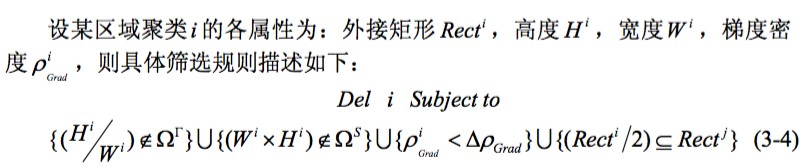
\includegraphics[width=0.618\textwidth]{image/2_5_2.jpg}    
    \label{logic}
\end{figure}
这里选择的是较为宽松的阈值范围,为了不把真的车牌误删。而选入的非车牌区域可以在精确定位时被舍弃。
\item
车牌区域精确定位。

对每个车牌候选区域,
\begin{enumerate}
\item
利用其梯度形态特征分割得到车牌精确的上下边界:
引起车牌上下边界不确定的主要因素是出租车下边的小车牌。对该候选区域进行水平梯度化、二值化、平滑去噪以及形态学膨胀之后得到b)图像。对该二值图像进行逐行水平扫描,找到引起宽度跳变的行数值,也就找到了大小车牌的交接点。
具体实现时,可以从下向上扫描,当首次找到当前行的 2/3 还大于前一扫描行的时候,停止扫描认定其即为交接点,删掉此行下面的所有区域。
\begin{figure}[H]
    \centering 
    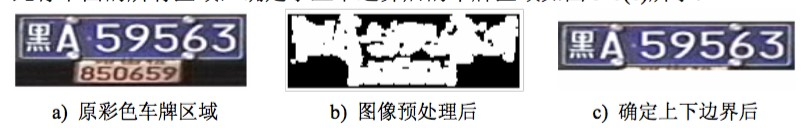
\includegraphics[width=0.618\textwidth]{image/2_5_3.jpg}    
    \label{logic}
\end{figure}
\item
对剩下部分彩色子图像进行 HSV 色彩变换
我国车牌包含了四种不同的配色方案,分别为蓝底白字(以下简称为蓝牌)、黄底黑字(黄牌)、白底黑字(白牌)和黑底白字(黑牌)。 作者通过查阅文献,得到这些颜色的HSV分量的分布范围:
\begin{figure}[H]
    \centering 
    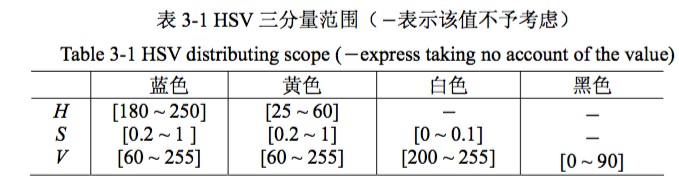
\includegraphics[width=0.618\textwidth]{image/2_5_4.jpg}    
    \label{logic}
\end{figure}
在寻找车牌左右边界时,我们以候选区域的高度作为标度创建平移窗口。 设候选区域高度为 H,宽度为 W,确定左右边界过程如下:
\begin{enumerate}
\item
当W ≤ H*6时,不用再确定车牌的左右边界,原候选区域即车牌的精确定位位置,只须以整个候选区域作为窗口判断出车牌的种类即可;
\item
当W > H*6时,按照宽度为 H*6,高度为 H 的窗口水平移动扫描候选区域,通过窗口平移找到每种配色方案概率值最大的窗口位置,比较这几种车牌配色的概率极值,最终取概率极值最大配色作为车牌种类,而该极值配色对应的窗口区域即为车牌的精确定位位置。 
\item
并且设定一个最小配色概率阈值,若当前极值配色概率值小于最小配色概率阈值,则认为该区域没有车牌,该区域为伪车牌。
\end{enumerate}
实验表明,该车牌检测和定位方法具有很好的实时性,且定位准确率高,为后面的车牌字符分割打下了良好的基础。不足之处在于在定位阶段过后留下了一些伪车牌区域没有被剔除。 
\end{enumerate}
\end{enumerate}
\subsection{开源系统EasyPR中用到的形态学方法与颜色定位法。}
\subsubsection{使用Sobel寻找垂直边缘}
Plate Detection的总流程如下:
\begin{figure}[H]
    \centering 
    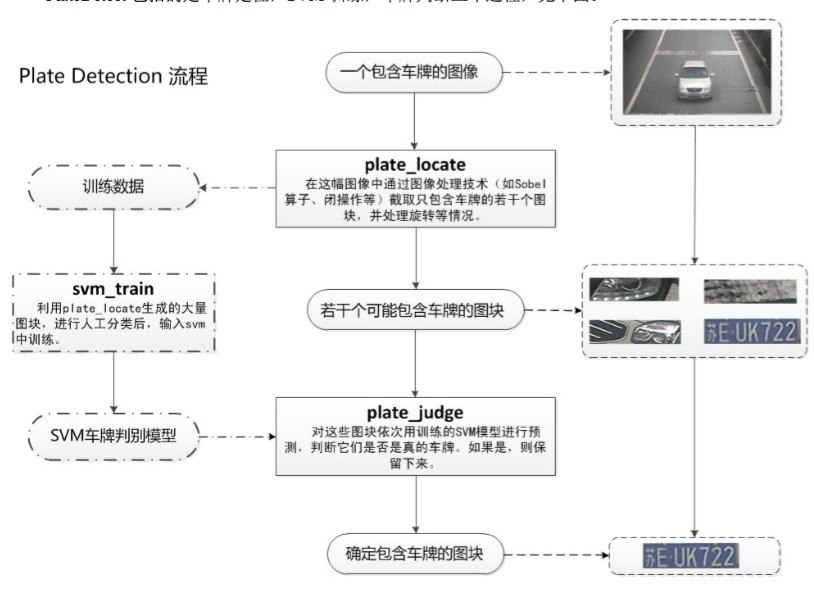
\includegraphics[width=0.618\textwidth]{image/2_6_1_1.jpg}    
    \label{logic}
\end{figure}
PlateLocate就是比较关键的车牌定位,流程如下:
\begin{enumerate}
\item
高斯模糊,去除干扰噪声,为边缘检测算法做准备。\\
高斯模糊中的半径也会给结果带来明显的变化。有的图片,高斯模糊半径过高或过低,车牌都无法定位。因此,高斯模糊的半径既不宜过高,也不能过低。作者对于近千张图片经过测试后得出的综合定位率最高的值为5。
\item
灰度化(OpenCV Sobel运算只能作用在灰度图像上)
\item
进行Sobel运算,得到一阶水平方向导数。用于垂直边缘检测。由于车子前端干扰性的水平边缘较多,这里只对水平方向求导,得到垂直边缘 。
\item
二值化
\item
闭操作,目的是将车牌字符区域连接成一个连通域,以便取轮廓。
闭操作就是对图像先膨胀,再腐蚀,闭操作的结果一般是可以将许多靠近的图块相连成为一个无突起的连通域。

其中,作者推荐矩形模板的宽度大于等于17,高度一般为3。因为中国车牌有一个特点,就是表示城市的字母与右边相邻的字符距离远大于其他相邻字符之间的距离。如果宽度设置不够大,左边的字符与右边的字符会断开:
\begin{figure}[H]
    \centering 
    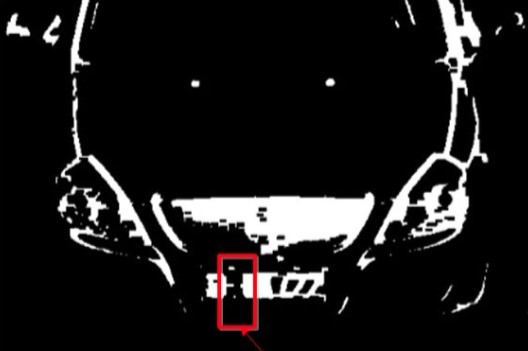
\includegraphics[width=0.618\textwidth]{image/2_6_1_2.jpg}    
    \label{logic}
\end{figure}
宽度过大也是不好的,因为它会导致闭操作连接不该连接的部分,例如下图的情况。
\begin{figure}[H]
    \centering 
    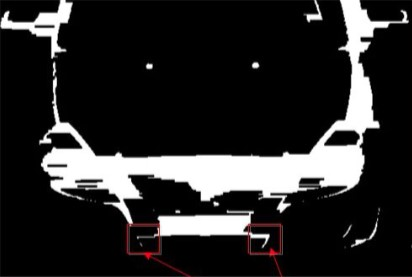
\includegraphics[width=0.618\textwidth]{image/2_6_1_3.jpg}    
    \label{logic}
\end{figure}
下图是合适宽度下的结果:
\begin{figure}[H]
    \centering 
    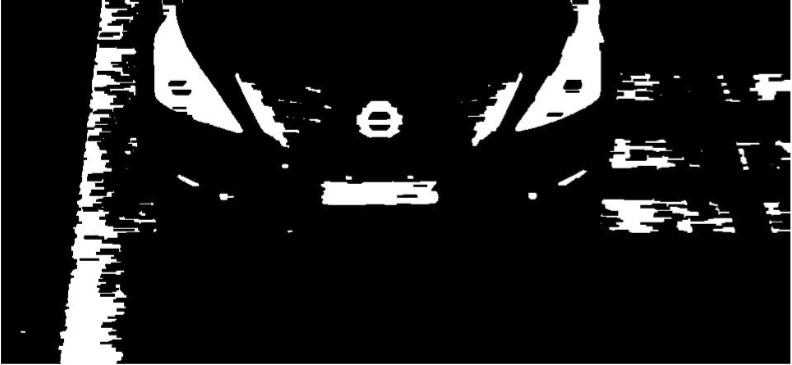
\includegraphics[width=0.618\textwidth]{image/2_6_1_4.jpg}    
    \label{logic}
\end{figure}
\item
求轮廓(OpenCV 函数 findContours)。将连通域的外围勾画出来,以便形成外接矩形(RotatedRect)。
\item
筛选。对轮廓求最小外接矩形,然后验证,不满足条件的淘汰。
尺寸判断:
中国车牌的一般大小是440mm*140mm,面积为440*140,宽高比为3.14。
使用如下方法判 断矩形是否是车牌:
\begin{enumerate}
\item
设立一个偏差率 error,根据这个偏差率计算最大和最小的宽高比 rmax、rmin。判断矩形的 r 是否满足在 rmax、rmin 之间。
\item
设定一个面积最大值 max 与面积最小值 min。判断矩形的面积 area 是否在 max 与 min 之间。
\end{enumerate}
以上两个条件必须同时满足,任何一个不满足都代表这不是车牌。

尺寸筛选后的结果:
\begin{figure}[H]
    \centering 
    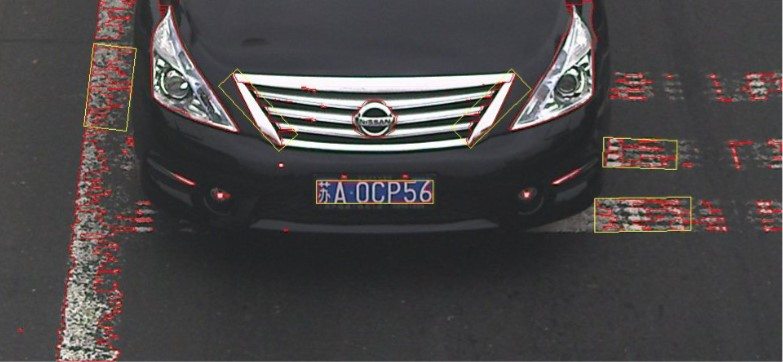
\includegraphics[width=0.618\textwidth]{image/2_6_1_5.jpg}    
    \label{logic}
\end{figure}
\item
角度判断与旋转。把倾斜角度大于阈值(如正负 30 度)的矩形舍弃。余下的矩形进行微小的旋转,使其水平。 最后得到了如下三个矩形:
\begin{figure}[H]
    \centering 
    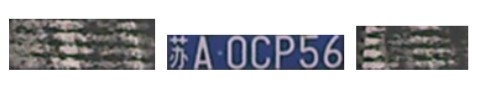
\includegraphics[width=0.618\textwidth]{image/2_6_1_6.jpg}    
    \label{logic}
\end{figure}
\item
统一尺寸。作者使用了136*36。
\end{enumerate}
整个过程流程图表示如下:
\begin{figure}[H]
    \centering 
    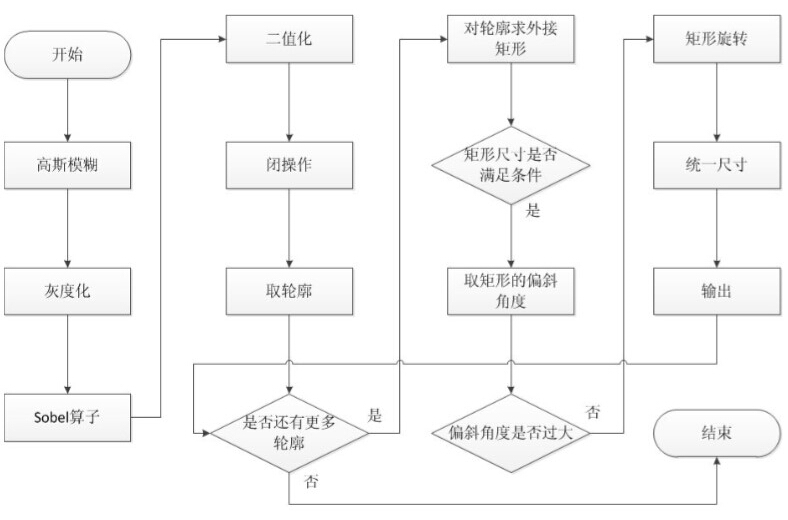
\includegraphics[width=0.618\textwidth]{image/2_6_1_7.jpg}    
    \label{logic}
\end{figure}
\subsubsection{颜色定位与偏斜扭正}
2.6.1节介绍的Sobel法最大的问题在于面对垂直边缘交错的情况下,无法准确定位车牌:
\begin{figure}[H]
    \centering 
    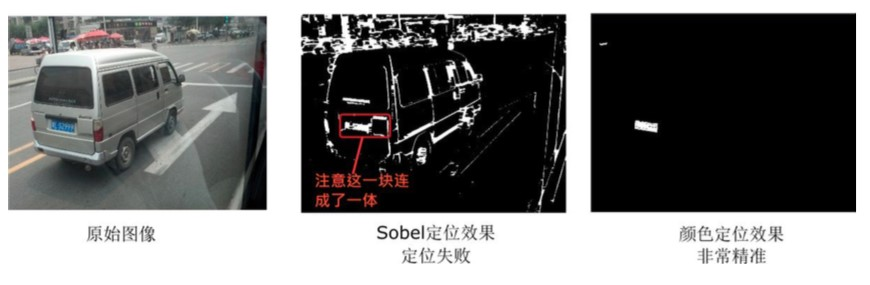
\includegraphics[width=0.618\textwidth]{image/2_6_2_1.jpg}    
    \label{logic}
\end{figure}
如果将颜色定位与 Sobel 定位加以结合的话,可以使车牌的定位准确率从 75\%上升到 94\%。 

这里选择使用HSV模型,对于颜色判断比较直观,例如蓝色的判断:
\begin{figure}[H]
    \centering 
    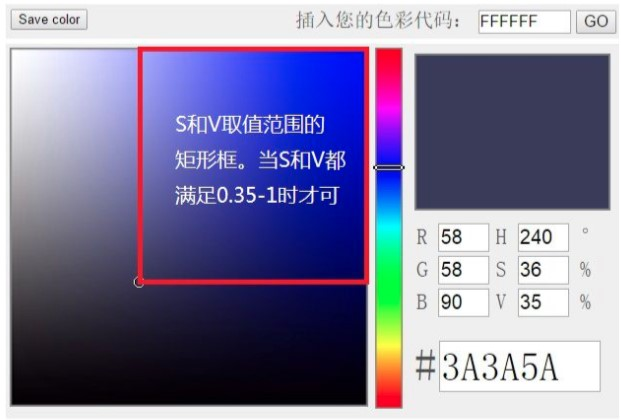
\includegraphics[width=0.618\textwidth]{image/2_6_2_2.jpg}    
    \label{logic}
\end{figure}
颜色定位的完整过程如下:
\begin{enumerate}
\item
将图像的颜色空间从 RGB 转为 HSV,由于光照的影响,对于图像使用直方图均衡进行预处理;
\item
依次遍历图像的所有像素,当 H 值落在 200-280 (蓝色),且 S 值与 V 值也落在 0.35-1.0之间,标记为白色像素,否则为黑色像素,这样,这里的蓝色区域就全部变成了白色像素,其余像素全为黑色。相当于使用了蓝色模板,筛选出了蓝色区域。

一幅图像需要进行一次蓝色模板的匹配,还要进行一次黄色模板的匹配,以此确保蓝色和黄色的车牌都被定位出来。 
\item
对仅有白黑两个颜色的二值图参照原先车牌定位中的方法,使用闭操作,取轮廓等方法将车牌的外接矩形截取出来做进一步的处理。

但是颜色定位不是万能的,面对光线不足、或者蓝色车身时,颜色定位很糟糕。这时可以再结合2.6.1节的Sobel方法。
\end{enumerate}

\subsubsection{EasyPR现阶段的车牌定位方式}
目前的新版本使用了颜色定位与 Sobel 定位结合的方式。首先进行颜色定位,然后根据条件使用 Sobel 进行再次定位,增加整个系统的适应能力。 

为了加强鲁棒性,Sobel 定位法可以用两阶段的查找。也就是在已经被 Sobel 定位的图块中,再进行 一次 Sobel 定位。这样可以增加准确率,但会降低速度。一个折衷的方案是让用户决定一个参数 m\_maxPlates 的值,这个值决定了你在一幅图里最多定位多少车牌。系统首先用颜色定位出候选车牌,然后通过 SVM 模型来判断是否是车牌,最后统计数量。如果这个数量大于你设定的参数,则认为车牌已 经定位足够了,不需要后一步处理,也就不会进行两阶段的 Sobel 查找。相反,如果这个数量不足,则继续进行 Sobel 定位。 
\begin{figure}[H]
    \centering 
    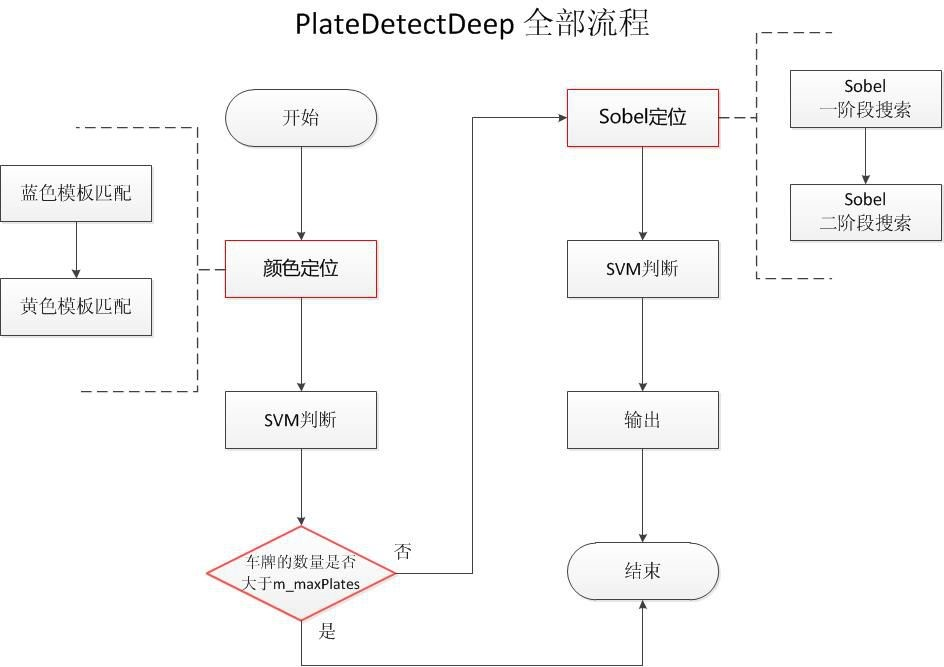
\includegraphics[width=0.618\textwidth]{image/2_6_3_1.jpg}    
    \label{logic}
\end{figure}
\subsubsection{偏斜扭转}
由于现实场景中拍摄到的车牌可能是倾斜的,也有可能是在斜视角下拍摄的,所以在这里需要调整,以便后面的字符分割与识别。整体流程如下图:
\begin{figure}[H]
    \centering 
    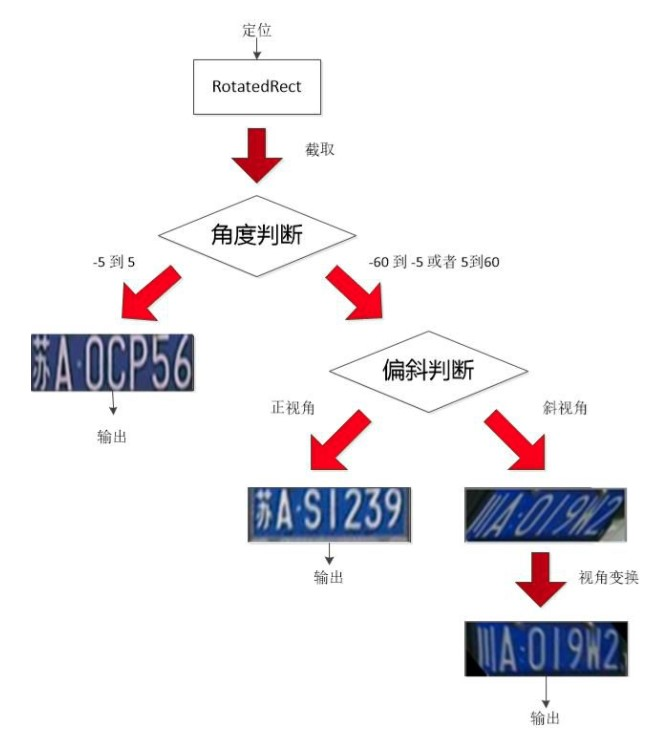
\includegraphics[width=0.618\textwidth]{image/2_6_4_1.jpg}    
    \label{logic}
\end{figure}
\begin{enumerate}
\item
ROI(region of interest)的截取。

使用RotatedRect的boundingRect()方法。返回一个RotatedRect的最小外接矩形,传递给Mat(Rect…)方法就可以截取出原图的ROI图块,获得对应的ROI图像(clone or copyTo)。
\item
扩大化旋转。

在获得RotatedRect时,我们就已经知道了车牌的倾斜角度,所以若角度较小,则直接输出,否则,需要作旋转操作。

为了防止旋转后车牌区域的一部分被截断:
\begin{figure}[H]
    \centering 
    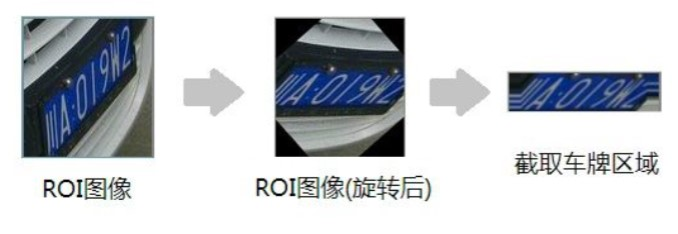
\includegraphics[width=0.618\textwidth]{image/2_6_4_2.jpg}    
    \label{logic}
\end{figure}
需要首先新建一个尺寸为原始图像1.5倍的新图像,接着把原始图像映射到新图像上,于是我们得到了一个显示区域(视框)扩大化后的原始图像。显示区域扩大以后,那些在原图像中没有值的像素被置了一个初值。 

接着调用 warpAffine 函数,使用新图像的大小作为目标图像的大小。warpAffine 函数会将新图像旋转,并用目标图像尺寸的视框去显示它。于是我们得到了一个所有感兴趣区域都被完整显示的旋转后图像。 

这样,我们再使用 getRectSubPix()函数就可以获得想要的车牌区域了:

\begin{figure}[H]
    \centering 
    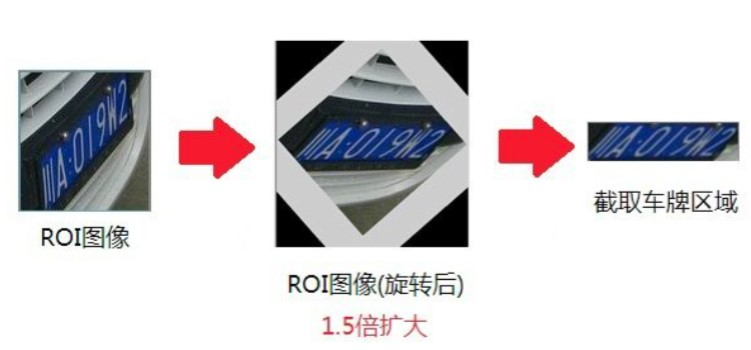
\includegraphics[width=0.618\textwidth]{image/2_6_4_3.jpg}    
    \label{logic}
\end{figure}
\item
偏斜判断。

为了判断二值化图像中白色的部分是平行四边形。一种简单的做法就是从图像中选择一些特定的行。计算在这个行中,第一个全为 0 的串的长度。从几何意义上来看, 这就是平行四边形斜边上某个点距离外接矩形的长度。 

假设我们选择的这些行位于二值化图像高度的$\frac{1}{4}$,$\frac{2}{4}$,$\frac{3}{4}$处的话,如果白色图形是矩形的话, 这些串的大小应该是相等或者相差很小的,相反如果是平行四边形的话,那么这些串的大小应该不等,并且呈现一个递增或递减的关系。通过这种不同,我们就可以判断车牌区域里的图形究竟是矩形还是平行四边形。 

偏斜判断的另一个重要作用就是,计算平行四边形倾斜的斜率,这个斜率值用来在下面的仿射变换中发挥作用。我们使用一个简单的公式去计算这个斜率,利用上面判断过程中使用的串大小,假设二值化图像高度的$\frac{1}{4}$,$\frac{2}{4}$,$\frac{3}{4}$处对应的串的大小分别为 len1, len2, len3,车牌区域的高度为 Height。 一个计算斜率 slope 的计算公式就是:
$$(len3-len1)/Height*2。$$ 

Slope 的直观含义见下图:
\begin{figure}[H]
    \centering 
    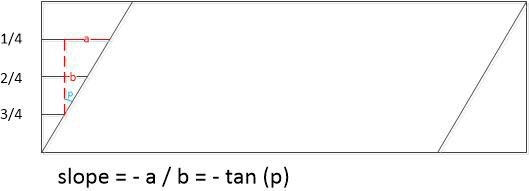
\includegraphics[width=0.618\textwidth]{image/2_6_4_4.jpg}    
    \label{logic}
\end{figure}

需要说明的,这个计算结果在平行四边形是右斜时是负值,而在左斜时则是正值。于是可以根据 slope 的正负判断平行四边形是右斜或者左斜。

在实践中,会发生一些公式不能应对的情况,例如像下图这种情况,斜边的部分区域发生了内凹或者外凸现象。这种现象会导致 len1, len2 或者 len3 的计算有误,因此 slope计算 也会不准。 
\begin{figure}[H]
    \centering 
    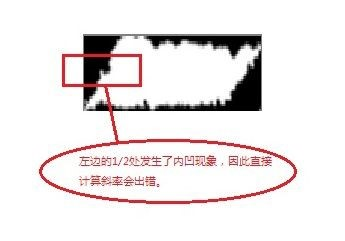
\includegraphics[width=0.618\textwidth]{image/2_6_4_5.jpg}    
    \label{logic}
\end{figure}
为了实现一个鲁棒性更好的计算方法,可以用$(len2-len1)/Height\times 4$ 与$(len3-len1)/Height \times 2$ 两者之间更靠近 tan(angle)的值作为 solpe 的值(在这里,angle 代表的是原来  RotataedRect 的角度)。 多采取了一个 slope 备选的好处是可以避免单点的内凹或者外凸。 
\item
仿射变化。

使用opencv的warpAffine函数,为保证新的视框中心能够正好与车牌的中心重合,我们可以选择偏移 xidff/2 长度。正如下图所显示的一样。 
\begin{figure}[H]
    \centering 
    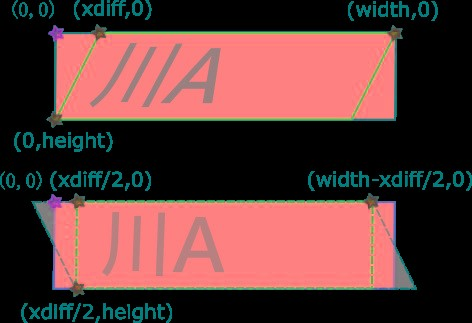
\includegraphics[width=0.618\textwidth]{image/2_6_4_6.jpg}    
    \label{logic}
\end{figure}
视框往右偏移的含义就是目标图像 Mat 的原点往右偏移。如果原点偏移的话,那么仿射后图像的三个 关键点的坐标要重新计算,都需要减去 xidff/2 大小。 

重新计算的映射点坐标为下:
plTri[0] = Point2f(0 + xiff, 0); \\
plTri[1] = Point2f(width - 1, 0); \\
plTri[2] = Point2f(0, height - 1); \\
dstTri[0] = Point2f(xiff/2, 0);
\\
dstTri[1] = Point2f(width - 1 - xiff + xiff/2, 0); \\
dstTri[2] = Point2f(xiff/2, height - 1); \\

效果图:
\begin{figure}[H]
    \centering 
    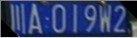
\includegraphics[width=0.618\textwidth]{image/2_6_4_7.jpg}    
    \label{logic}
\end{figure}
偏斜扭正全过程:
\begin{figure}[H]
    \centering 
    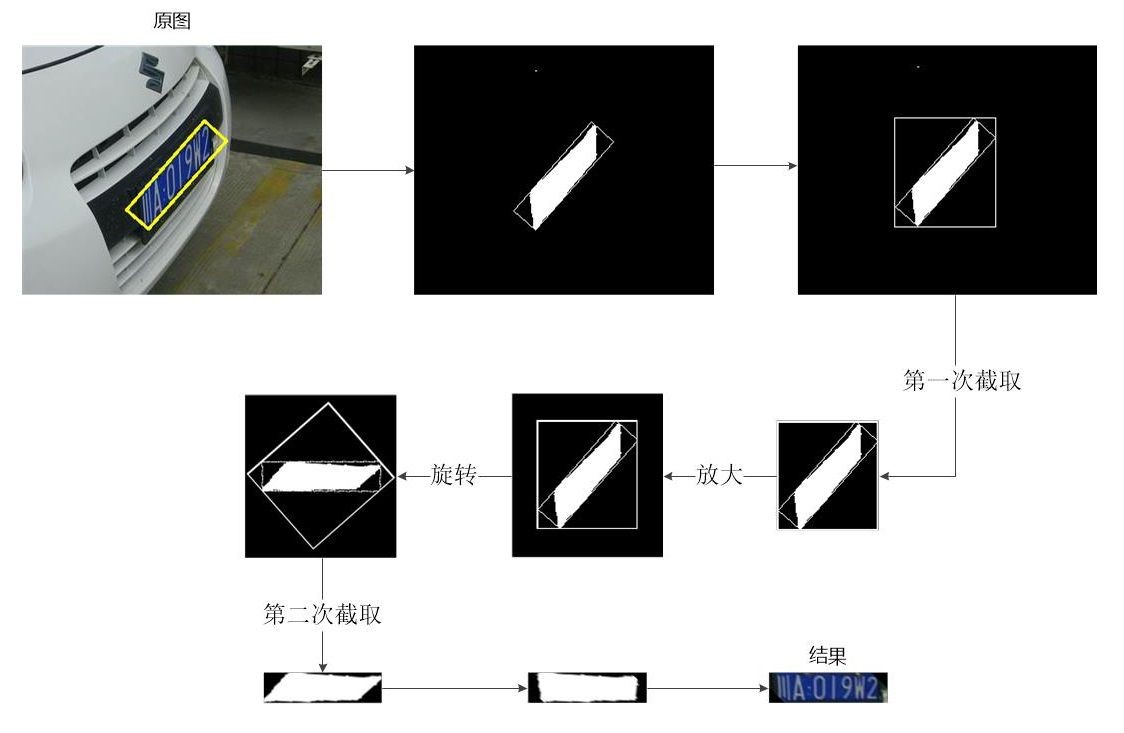
\includegraphics[width=0.618\textwidth]{image/2_6_4_8.jpg}    
    \label{logic}
\end{figure}
\end{enumerate}
\subsubsection{SVM训练}
流程如下图:
\begin{figure}[H]
    \centering 
    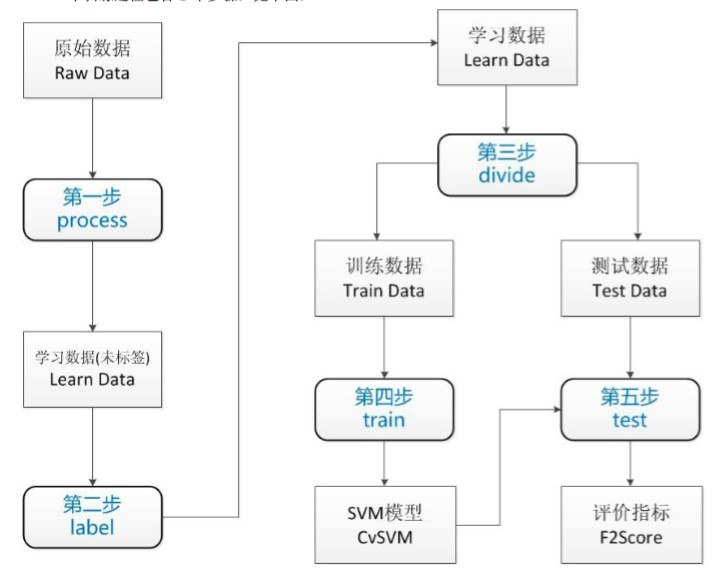
\includegraphics[width=0.618\textwidth]{image/2_6_5_1.jpg}    
    \label{logic}
\end{figure}
作者使用了opencv相关函数,在这里不赘述了。
值得一提的是,人工对数据进行标签是一件非常耗时的事情,于是作者提出了“逐次迭代自动标签法”:

方法核心很简单。就是假设你有 3000 张未分类的图片。你从中选出 1\%,也就是 30 张出来,手工给它们每个图片进行分类工作。如今你有了 30 张贴好标签的数据了,下一步你把它直接输入到 SVM 模型中训练,获得了一个简单粗旷的模型。之后,你从图片集中再取出 3\%的图片,也就是 90 张,然后用刚训练好的模型对这些图片进行预测,根据预测结果将它们自动分到 hasplate 和 noplate 文件夹下面。 分完以后,你到这两个文件夹下面,看看哪些是预测错的,把 hasplate 里预测错的移动到 noplate 里, 反之,把 noplate 里预测错的移动到 hasplate 里。 

接着,你把一开始手工分类好的那 30 张图片,结合调整分类的 90 张图片,总共 120 张图片再输入 svm 模型中进行训练。于是你获得一个比最开始粗旷模型更精准点的模型。然后,你从 3000 张图片中再 取出 6\%的图片来。用这个模型再对它们进行预测,分类.... 

以上反复。你每训练出一个新模型,用它来预测后面更多的数据,然后自动分类。这样做最大的好处就是你只需要移动那些被分类错误的图片。其他的图片已经被正 确的归类了。注意,在整个过程中,你每次只需要对新拿出的数据进行人工确认,因为前面的数据已经分好类了。因此,你最好使用两个文件夹, 一个是已经分好类的数据,另一个是自动分类数据,需要手工确认的。这样两者不容易乱。 

每次从未标签的原始数据库中取出的数据不要多,最好不要超过上次数据的两倍。这样可以保证你的 模型的准确率稳步上升。如果想一口吃个大胖子,例如用 30 张图片训练出的模型,去预测 1000 张数据,那最后结果跟你手工分类没有任何区别了。 
